%\documentclass[conference]{IEEEtran}
%\IEEEoverridecommandlockouts
%\documentclass[sigconf]{acmart}
%\let\Bbbk\relax %% fix bug
\documentclass[twocolumn,10pt]{article}
\usepackage[utf8]{inputenc}

% =======================
\usepackage{amssymb}
\usepackage{amsmath}
\usepackage{amstext}
\usepackage{amsopn}
%\usepackage{algorithmic}
\usepackage{graphicx}
\usepackage{textcomp}
\usepackage{xcolor}

\usepackage{textcomp}

\usepackage{boxedminipage}
\usepackage{enumerate}
\usepackage{multirow}
\usepackage{url}
\usepackage{times}
\usepackage{version}
% \usepackage[pdftex]{graphicx}
\usepackage{graphicx} 
\usepackage{epsfig}
\usepackage{epsf}
%\usepackage{graphics}
\usepackage{caption}
\usepackage{subfigure}
\usepackage{algorithm}
\usepackage{algpseudocode}
%\PassOptionsToPackage{bookmarks={false}}{hyperref}
%%%%%%%%%%%%
\usepackage{comment}
\usepackage{multicol}
\usepackage{booktabs}
\usepackage{dblfloatfix}
\usepackage{hyperref}
% ==========================
%\usepackage[a4paper, margin = 2.5cm]{geometry}

\algrenewcommand\alglinenumber[1]{\footnotesize #1}
\algnewcommand\algorithmicassume{\textbf{Assumption:}}
\algnewcommand\Assume{\item[\algorithmicassume]}

\AtBeginDocument{%
  \providecommand\BibTeX{{%
    \normalfont B\kern-0.5em{\scshape i\kern-0.25em b}\kern-0.8em\TeX}}}

\begin{document}

\title{The Accuracy of KNN, SVM, SVDD, neural network and DBSCAN, k-means for Determining the Cancer by Gene-expression Signatures And the Arrhythmia Types}

\author{Hsieh Cheng-Han, Hsu Ting-Hao, Sun Shih-Yu, Lu Che-Yuan, Huang Chia-Yen}
\date{May 2023}
\maketitle

\section*{Abstract}
Nowadays, using machine to give an early diagnosis of a cancer type is widely studied. 
In this paper, based on the gene-expression dataset on Synapse.org, we compare the performance of machine 
learning techniques, including data preprocessing, e.g., Principal components analysis (PCA), Autoencoder 
(AE), classification, e.g., k-nearest neighbors (KNN), support vector machine (SVM), neural network (NN), 
and clustering for dealing with unknown types, e.g., k-means, density-based spatial clustering of 
applications with noise (DBSCAN). 

The result of gene dataset shows that, with PCA reducing the dimension of the dataset to 32, use KNN for 
classifying the known types, and finally apply DBSCAN on the remaining data, the accuracy of predicting 
can reach about 94\%, which beats the other methods out. In the other way, the result of arrhythmia 
dataset shows that, with raw data, use KNN and k-means, the highest accuracy of predicting can reach about 
53\%.

The source code can be found in \href{https://github.com/OEmiliatanO/CSE\_data\_mining}{https://github.com/OEmiliatanO/CSE\_data\_mining}.

\section{Introduction}
\label{sec:Introduction}
Over the years, machine learning methods for early predict various disease are widely used in medical field. 
\cite{kourou2015machine} \cite{cruz2006applications} From diabetes \cite{kavakiotis2017machine}, 
heart disease \cite{learning2017heart}, to lung adenocarcinoma \cite{huang2020machine} etc., machine learning 
methods is universally studied attributed to the promising perspective. With a well-built database of disease 
and a well-choose combination of machine learning mathods, within seconds, a machine may determine the type of 
disease that this person may have by collecting the data from the person, and thereby achieve the goal of 
personalized medicine. As a result, machine learning methods have become a popular tool for medical researchers. 

In real application, besides from the konwn diseases in the train data, there're numerous unkown types of diseases. 
When a new type of disease appears, how shall the machine results? In ideal situation, this new type of disease should be 
reported as an unkonwn type, which can be done by the combination of classification and clustering. 
However, how to choose the proper machine learning methods is a hot potato, since the different combinations 
of machine learning methods have different performance. 

In this work, the dataset on Synapse.org is used, which contains 20531 RNA sequences and 3 types of cancer 
in the train data, i.e., kidney renal clear cell carcinoma (KIRC), breast invasive carcinoma (BRCA), 
lung adenocarcinoma (LUAD), and 2 new types in test data, i.e., colon adenocarcinoma (COAD), 
prostate adenocarcinoma (PRAD). And also, the dataset of arrhythmia is included, which caintains
8 types in train data, and 5 new types in test data. To find out which techniques is more suitable to fit 
these two datasets, this work examines the the accuracy of the combinations of some major machine 
learning techniques, including PCA, AE, KNN, SVM, NN, k-means, DBSCAN. 

\section{Related works}
\label{sec:Related works}

\subsection*{Data preprocess}

\bf{Autoencoder (AE)}: \rm{An} AE is a type of neural network used for unsupervised 
learning and dimensionality reduction. It is designed to learn efficient representations or encodings of 
input data by training the network to reconstruct its own inputs. The AE consists of an encoder 
and a decoder. The encoder compresses the input data into a lower-dimensional representation, often called 
the latent space or code. The decoder then aims to reconstruct the original input data from this compressed 
representation. By learning a compact representation of the input data, AEs can capture important features 
and discard noise or irrelevant information \cite{lu2013speech}. This makes them effective in tasks such as 
image \cite{zhang2018better} \cite{lore2017llnet} \cite{cheng2018deep} or text classification \cite{xu2017variational} 
\cite{xu2019semisupervised}, where reducing the dimensionality of the data can improve performance.

\bf{Principal components analysis (PCA)}: \rm{PCA} is a statistical technique used for dimensionality 
reduction and data exploration. It aims to transform a dataset with a large number of variables into 
a lower-dimensional space while preserving the most important information. PCA accomplishes this by 
identifying the principal components, which are linear combinations of the original variables. 
Applications of PCA span various fields, including image \cite{ma2019dimension} \cite{YANG20021997} 
and signal processing \cite{6497960} \cite{castells2007principal}, genetics \cite{reich2008principal} 
\cite{novembre2008interpreting}. It is particularly useful in scenarios where the dataset is 
high-dimensional and the interpretation and visualization of the data are challenging.

\bf{Standardization and Interpolation}: \rm{With} simple interpolation, the dataset size can be easily increased. To ensure that the new produced data would not lower the correctness and precsion of the dataset, standardization to the origin dataset is required.\cite{chen2022doublemix} has used simple interpolation to achieve data augmentation with great outcome. With standardization and interpolation, we earn enough data for the latter machine learning.

\subsection*{Classification algorithm}

\bf{k-nearest neighbors (KNN) classification algorithm}: \rm{The} KNN classification algorithm is a 
supervised learning method which is first developed by Fix and Hodges \cite{10.2307/1403797}. The idea 
of KNN is based on the idiom, "birds of a feather flock together". By picking the $k$-nearest neighbors 
of a data point, the unkonwn class label can be determined. Lots of works \cite{6528591} \cite{8276012} 
\cite{vijayan2014study} show the fact that KNN performs  well for prediction of diabetes disease.

\bf{support vector machine (SVM)}: \rm{Given} a set of training datas, where each data is labeled as a 
binary class, such as $0$ and $1$, SVM training algorithm creates a model that assigns new examples to 
the binay labels by making it a non-probabilistic binary linear classifier. In addition, accroding to 
\cite{amari1999improving} \cite{hofmann2006support}, SVM can also use a method called kernel trick to 
effectively perform non-linear classification by implicitly mapping its inputs into a high-dimensional 
feature space. 
The idea of kernel trick is transform the data into higher dimension. In ideal situation, the dataset 
which is not linear separable becomes linear separable. Fig~\ref{fig:SVM_kernel_trick} illurates this 
case. 

\begin{figure}[htb]
    \centering
    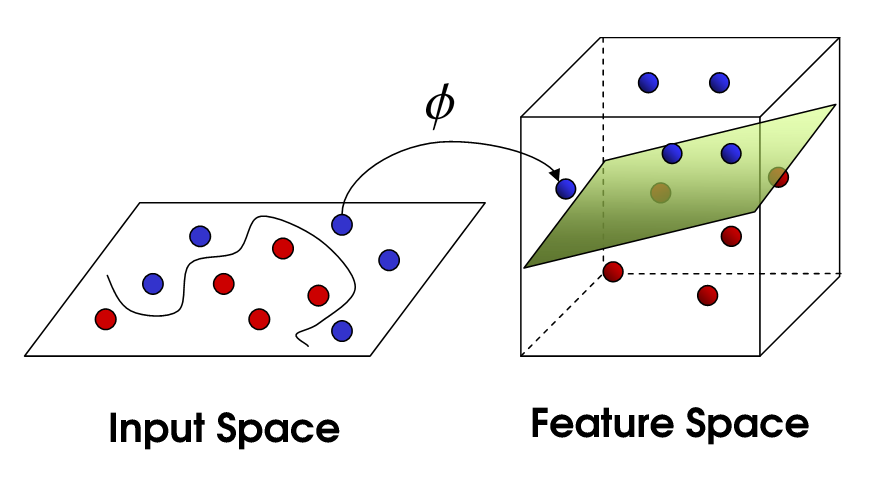
\includegraphics[scale=0.25]{assets/SVM_kernel_trick.png}
    \caption{An example of SVM kernel trick}
    \label{fig:SVM_kernel_trick}
\end{figure}

\bf{neural network (NN)}: \rm{Neural} network have been used in many fields to deal with intricate datas. 
With input layer, hidden layer and output layer constructed by neurons, each data in dataset is processed 
while passing through neurons, layer by layer. After the processing, the outcome can be used to predict. 
Using back propogation, the accuracy of predictions increase in each training. In order to construct the 
hidden layer more efficient, NAS(Neural Arcitecture Searching) is used to search suitable structure for 
hidden layer, increasing the accuracy. According to \cite{Gadekallu2020}\cite{Beghriche2021}, many neural 
network have been constructed and trained already, with high efficiency and accuracy in prediction of 
diabetes.


\bf{naive bayes classifier}: \rm{naive Bayes classifier} as its name suggest, is a machine learning method base on Bayesian 
theorem, this model will statistic each data and find all conditional probability of each event occurring if each outcome holds. 
And finally when it is asked to predict the result, the model will evaluate the data which requist provide and find the most 
likely outcome according to the conditional probability it just recorded. 

\subsection*{Clustering algorithm}

\bf{k-means}: \rm{K-means} is a popular and easily implemented clustering method in machine learning and 
data analysis. With $n$ data points in a dataset, k-means algorithm partition them into $k$ distinct 
clusters. The algorithm works iteratively and converges to a solution by minimizing the sum of squared 
distance between the data points and the center of their cluster. K-means is a useful algorithm for 
clustering data, which is widely applied on many researches, e.g. \cite{oyelade2010application}, 
\cite{NIDHEESH2017213}, \cite{kadhm2018accurate}.

\bf{Density-based spatial clustering of applications with noise (DBSCAN)}: \rm{DBSCAN} is a data clustering 
algorithm proposed by Ester et al. \cite{10.5555/3001460.3001507} DBSCAN is particularly effective in 
discovering clusters of arbitrary shapes and handling noise in the data. Unlike k-means need user specify 
how many clusters, DBSCAN determine the clusters and noise automatically by the density of data points. 
This characteristic makes it particularly useful when addressing the datasets where the number of cluster 
is unkonwn. DBSCAN is the major clustering algorithm in machine learning field, since the ability to 
discover the number of clusters automatically. And the variants of DBSCAN \cite{6814687} is also developed widely. 

\bf{Support Vector Data Description(SVDD)}:  \rm{SVDD} is an unsupervised learning algorithm used for one-class classification or outlier detection. It defines a hypersphere in the feature space to include some specific data to classify one class from other classes. With Deep SVDD, which is the variant of the SVDD which utilize the deep learning, more precise classification can be achieved providing only one class data.\cite{perera2021oneclass} give us the precise explanation how to train a model to classify data with only one class.

\bf{Nearest neighbor chain(NN-Chain)}: \rm{NN-Chain} is data clustering algorithm developed by Jean-Paul Benzécri and J. Juan\cite{Benzécri1982}. This method cluster the data by merge mutual nearest neighbors nodes to one node, and repeat the same action until the goal clustering number is achieved. While the distance can be earned by the normal Euclidean distance, some distance approach is used in the algorithm as well to suit some specific data.\cite{10.1093/comjnl/26.4.354}\cite{müllner2011modern}. NN-Chain is one of the hierarchical clustering algorithm which is likely to be presented in tree-like data structure.
\section{Main Process}
  The pesudo code of the proposed algorithm to process the dataset is shown below and Fig~\ref{fig:Main_Algo} 
  illurates the process of this algorithm:
  \begin{algorithm}
    \caption{The Main Algorithm}\label{alg:main}
    \begin{algorithmic}[1]
      \Require $\text{Dataset}$
      \State $\text{Data}, \text{Labels} \gets \text{Dataset}$
      \State $\text{Data}' \gets \text{preprocess}(\text{Data})$
      \State $\text{Konwns}, \text{Unkonwns} \gets \text{classify}(\text{Data}')$
      \State $\text{Clusters} \gets \text{clustering}(\text{Unkonwns})$
      \State $\text{Accuracy} \gets \text{calacc}((\text{Konwns}, \text{Clusters}), \text{Labels})$
    \end{algorithmic}
  \end{algorithm}

  \begin{figure}[htb]
    \centering
    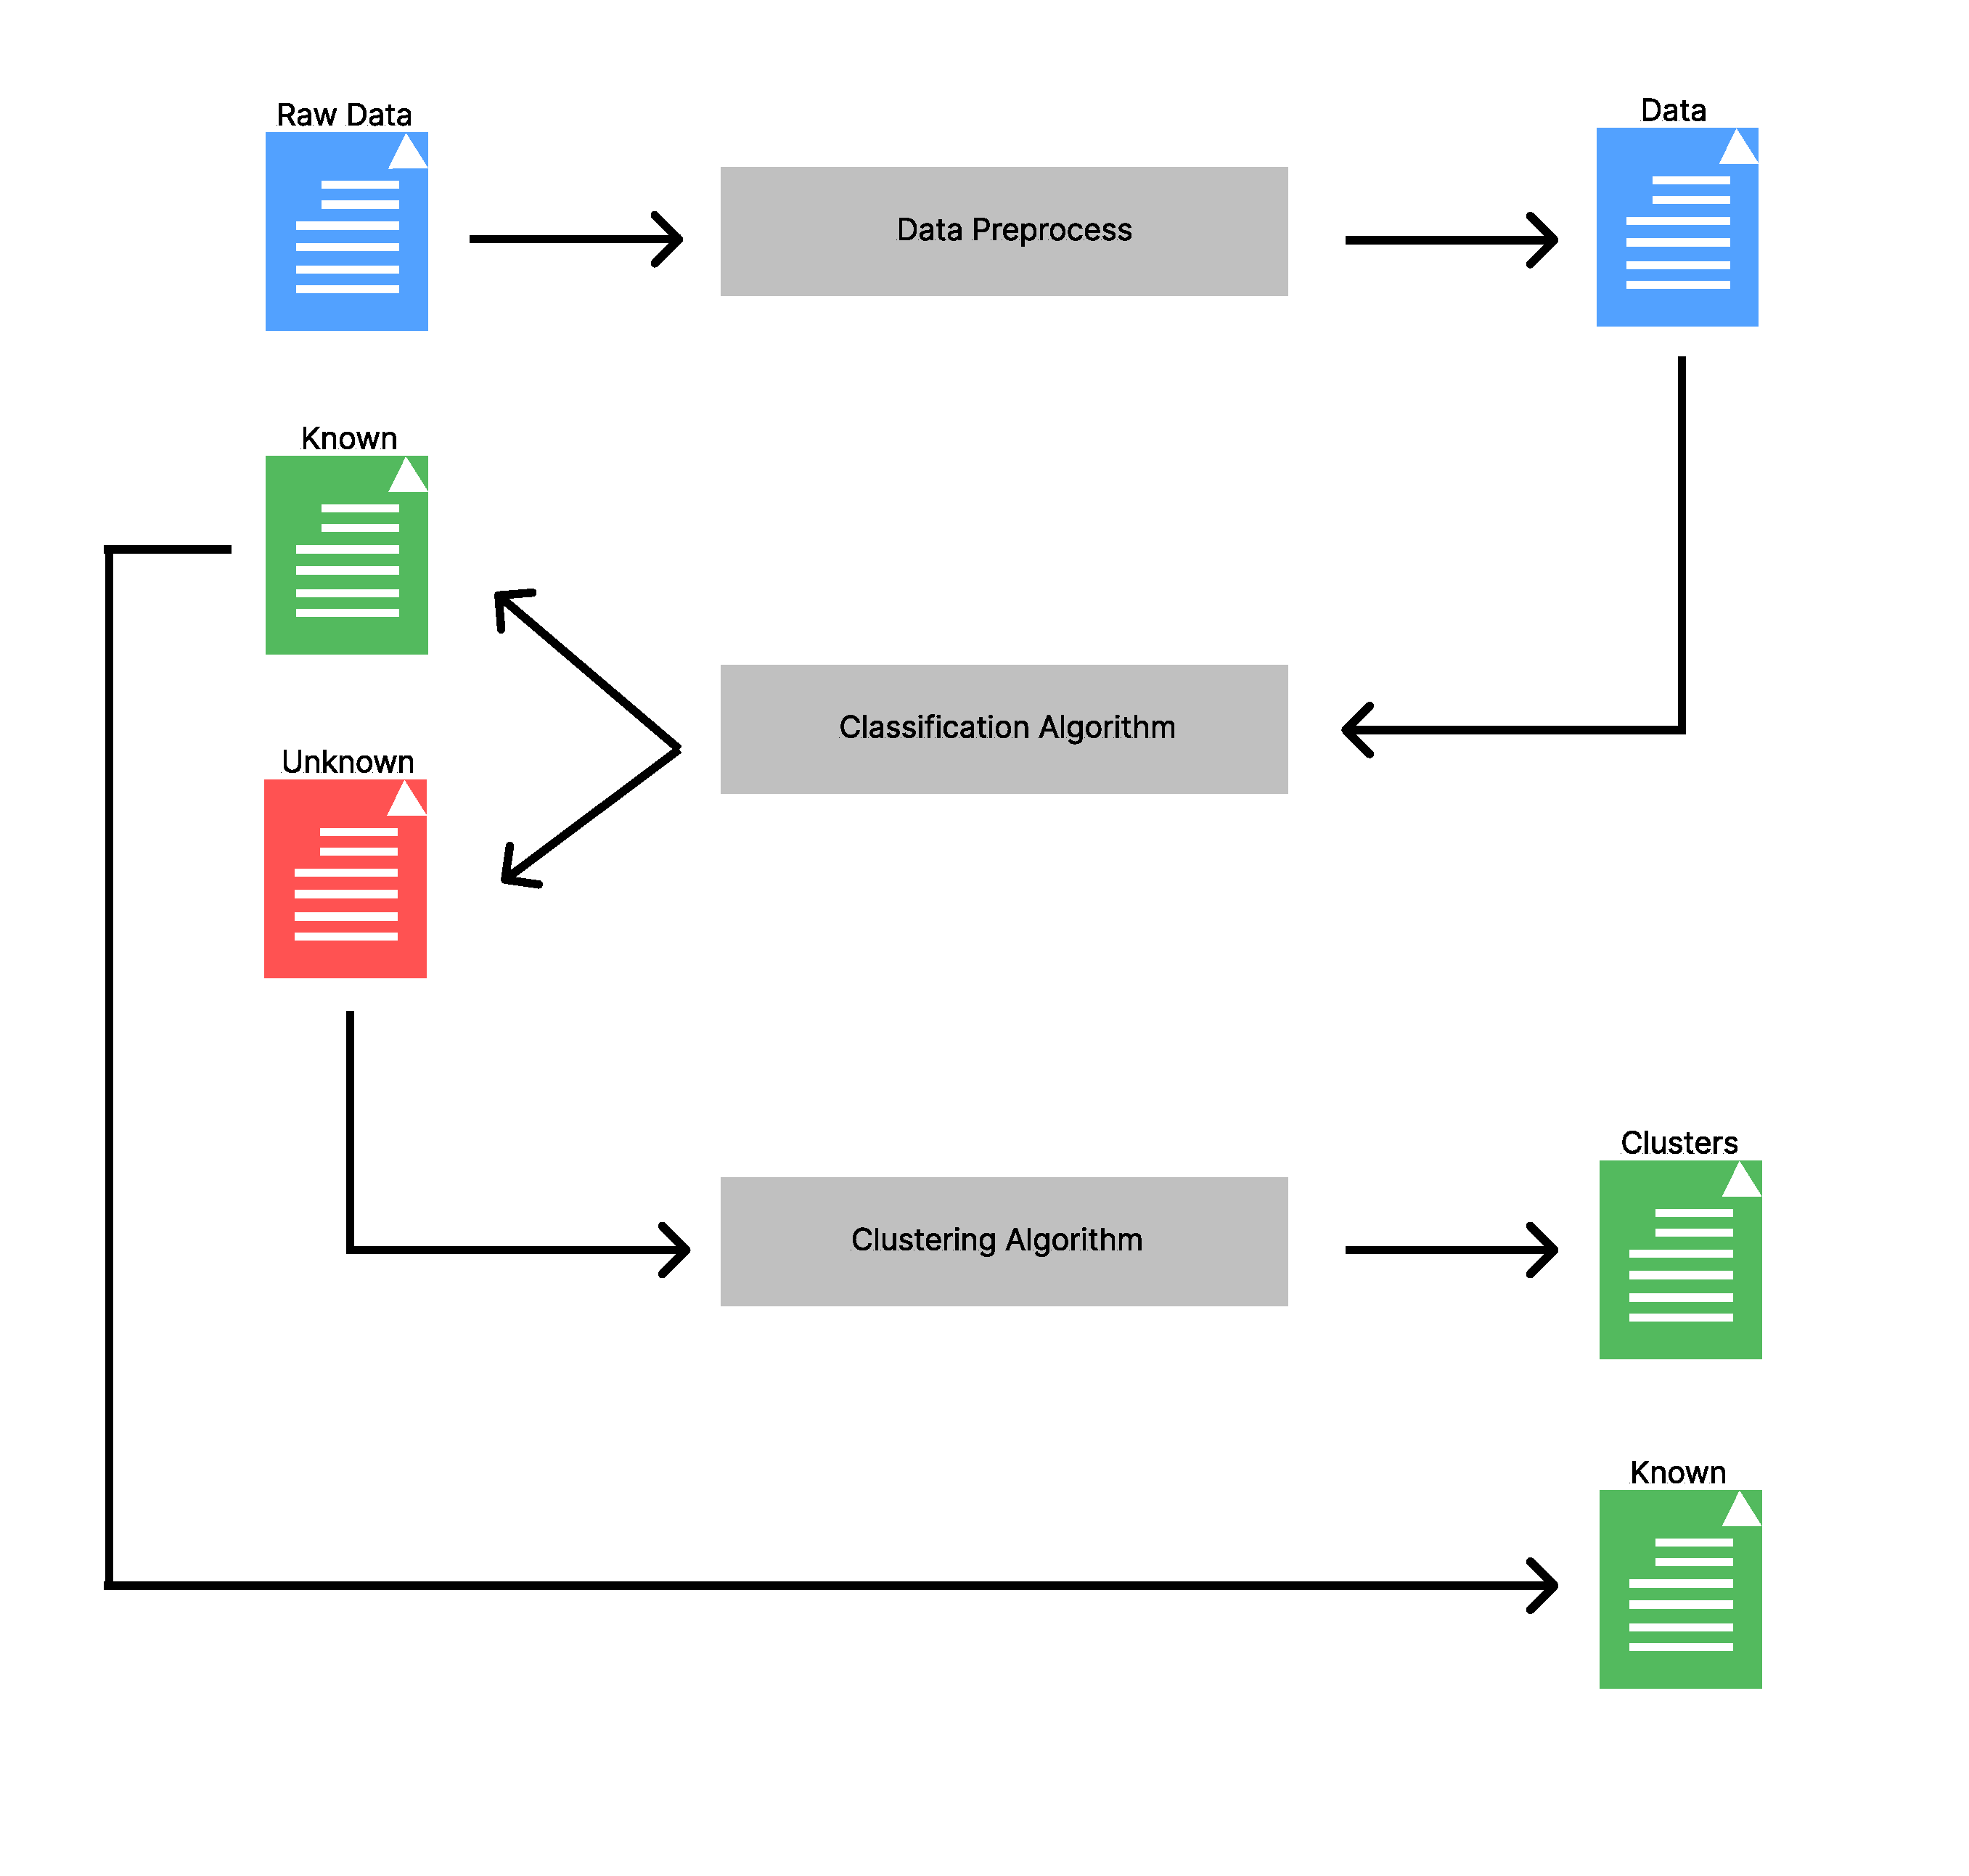
\includegraphics[scale=0.20]{assets/Main_Algo.pdf}
    \caption{A figure about the main algorithm}
    \label{fig:Main_Algo}
  \end{figure}

  First, preprocess the dataset, e.g. normalize, apply PCA, apply AE. Second, classify the data after preprocessing. 
  In the experiment, we use PCA and AE to reduce the dimension down to 32 and 30 in arrhythmia dataset and gene 
  expression cancer RNA-Seq dataset, respectively. 
  With this step, the konwn types and the unknown types will be separated by a certain criterion. This criterions will 
  be varied depending on the classification algorithm. For KNN, the criterion is distance and probability. More specifically, 
  assume a data point $x$, and the k-nearest data points are $p_1,...,p_k$. Only those points whose distance between 
  $x$ smaller than $L$ will be marked valid. Denote the valid data points as $p'_1,...p'_n$, and the corresponding 
  labels are $l_1,...,l_n$. If this data point satisifies Eq~\ref{eqn:KNN_prob}, mark it as unkown type.
  \begin{equation}
    \label{eqn:KNN_prob}
    \frac{\arg\max_{t\in\text{types}\{N(t)\}}}{n}<P
  \end{equation}
  where $P$ is a manunally set probability and $N(t)$ is the number of type $t$ in those $n$ valid data points.
  
  As for SVM, the criterion born in the designed. Since SVM is meant to be a binary classifier, the SVM classification 
  algorithm must be redesigned. As shown in Algo~\ref{alg:SVMs}. 
  \begin{algorithm}[h]
    \caption{The SVM Multi-classification Algorithm}\label{alg:SVMs}
    \begin{algorithmic}[1]
      \Require $\text{Train Data, Labels, Test Data}$
      \Assume $\text{Length}(\text{Train Data})=\text{Length}(\text{Labels})=N,\text{Length}(\text{Test Data})=M$
      \For{$t \text{ in Known Types}$}
        \For{$i \text{ in }[1,N]$}
          \If{$\text{Labels}[i]\neq t$}
            \State $\text{Labels}'[i] = +1$
          \Else
            \State $\text{Labels}'[i] = -1$
          \EndIf
        \EndFor
        \State $\text{SVM}[t].\text{fit}(\text{Train Data}, \text{Labels}')$
      \EndFor
      \For{$t \text{ in Known Types}$}
        \For{$i\text{ in }[1,M]$}
          \If{$\text{SVM}[t].\text{predict}() = +1$}
            \State $\text{Test Labels}[i] = t$
          \Else
            \State $\text{Test Labels}[i] = \text{UNKNOWN}$
          \EndIf
        \EndFor
      \EndFor
    \end{algorithmic}
  \end{algorithm}

  On the other hands, neural network classifier has another criterion. First, train a neural network that classify the 
  "konwn" and "unknown". Here "kown" means the types in train data, and "unkown" means the reverse. Then train the other 
  neural network to classify the "konwn" data. The detail is in Algo~\ref{alg:NN}.
  \begin{algorithm}[tb]
    \caption{Neural Network Classification}\label{alg:NN}
    \begin{algorithmic}[1]
      \Require $\text{Train Data, Labels, Test Data}$
      \Assume $\text{Length}(\text{Train Data})=\text{Length}(\text{Labels})=N,\text{Length}(\text{Test Data})=M$
      \State{$\text{Binary NN}.\text{train(Train Data, Labels)}$}
      \State{$\text{Mutli-Classification NN}.\text{train(Train Data, Labels)}$}
      \State{$\text{Just Knowns, Unkonwns}=\text{Binary NN}.\text{predict}(\text{Test Data})$}
      \State{$\text{Knowns}=\text{Mutli-Classification NN}.\text{predict}(\text{Just Knowns})$}
    \end{algorithmic}
  \end{algorithm}
  During the known-unknown classification, the SVDD is used. First define a model , input every data into it to get the outcome, then use the mean of the outcome as the center of the hypersphere. Then, train the model to make every data in the dataset approach to the center of the hypersphere as close as possible. After training, we can get the radius of the hypersphere, which can be define according to the outcome of the model. Using the radius, we can classify the data to "known", if the distance between the center and the data is less than or equal to the radius, or to "unknown" otherwise.

  When it comes to Naive Bayes classifier, Assume there are N known types. Denotes the N Bayes classifiers recognizing each
  type of known types as BC_1, BC_2, ..., BC_N. For each test data, let BC_1 determine whether it belongs to     type 1, if
  it does, mark it as type 1 and try classifying next test data, otherwise, BC_2 will determine whether it belongs to class_2
  or not, and so on. If all Bayes classifiers results false, namely, the data doesn't belong to     any known types, marks it
  as unknown type.
  
  After classifying, the konwn types and unkonwn types are separated. The data marked as unkonwn types will be thrown 
  into clustering algorithm, e.g., DBSCAN, k-means. Subsequently, the process is completed.

\section{Experiment result}
  The experiment result of arrhythmia dataset is shown in Table~\ref{table:Arrhythmia_result}. And the result of gene 
  expression cancer RNA-Seq data set is in Table~\ref{table:gene_expression_result}. 

  From the result, the fact that SVM performs worse than KNN can be seen. The main reason is because the mult- 
  classification SVMs method designed here can't separate well in most of types. Fig~\ref{fig:SVM_fail} illurates the 
  situation. For type 1 SVM, the negative/positive classification makes the data hard to separate, and also for type 
  2, 3, etc. This happens even when the kernel trick is applied, though the kernel trick sometimes ease the pain. 
  \begin{figure}[htb]
    \centering
    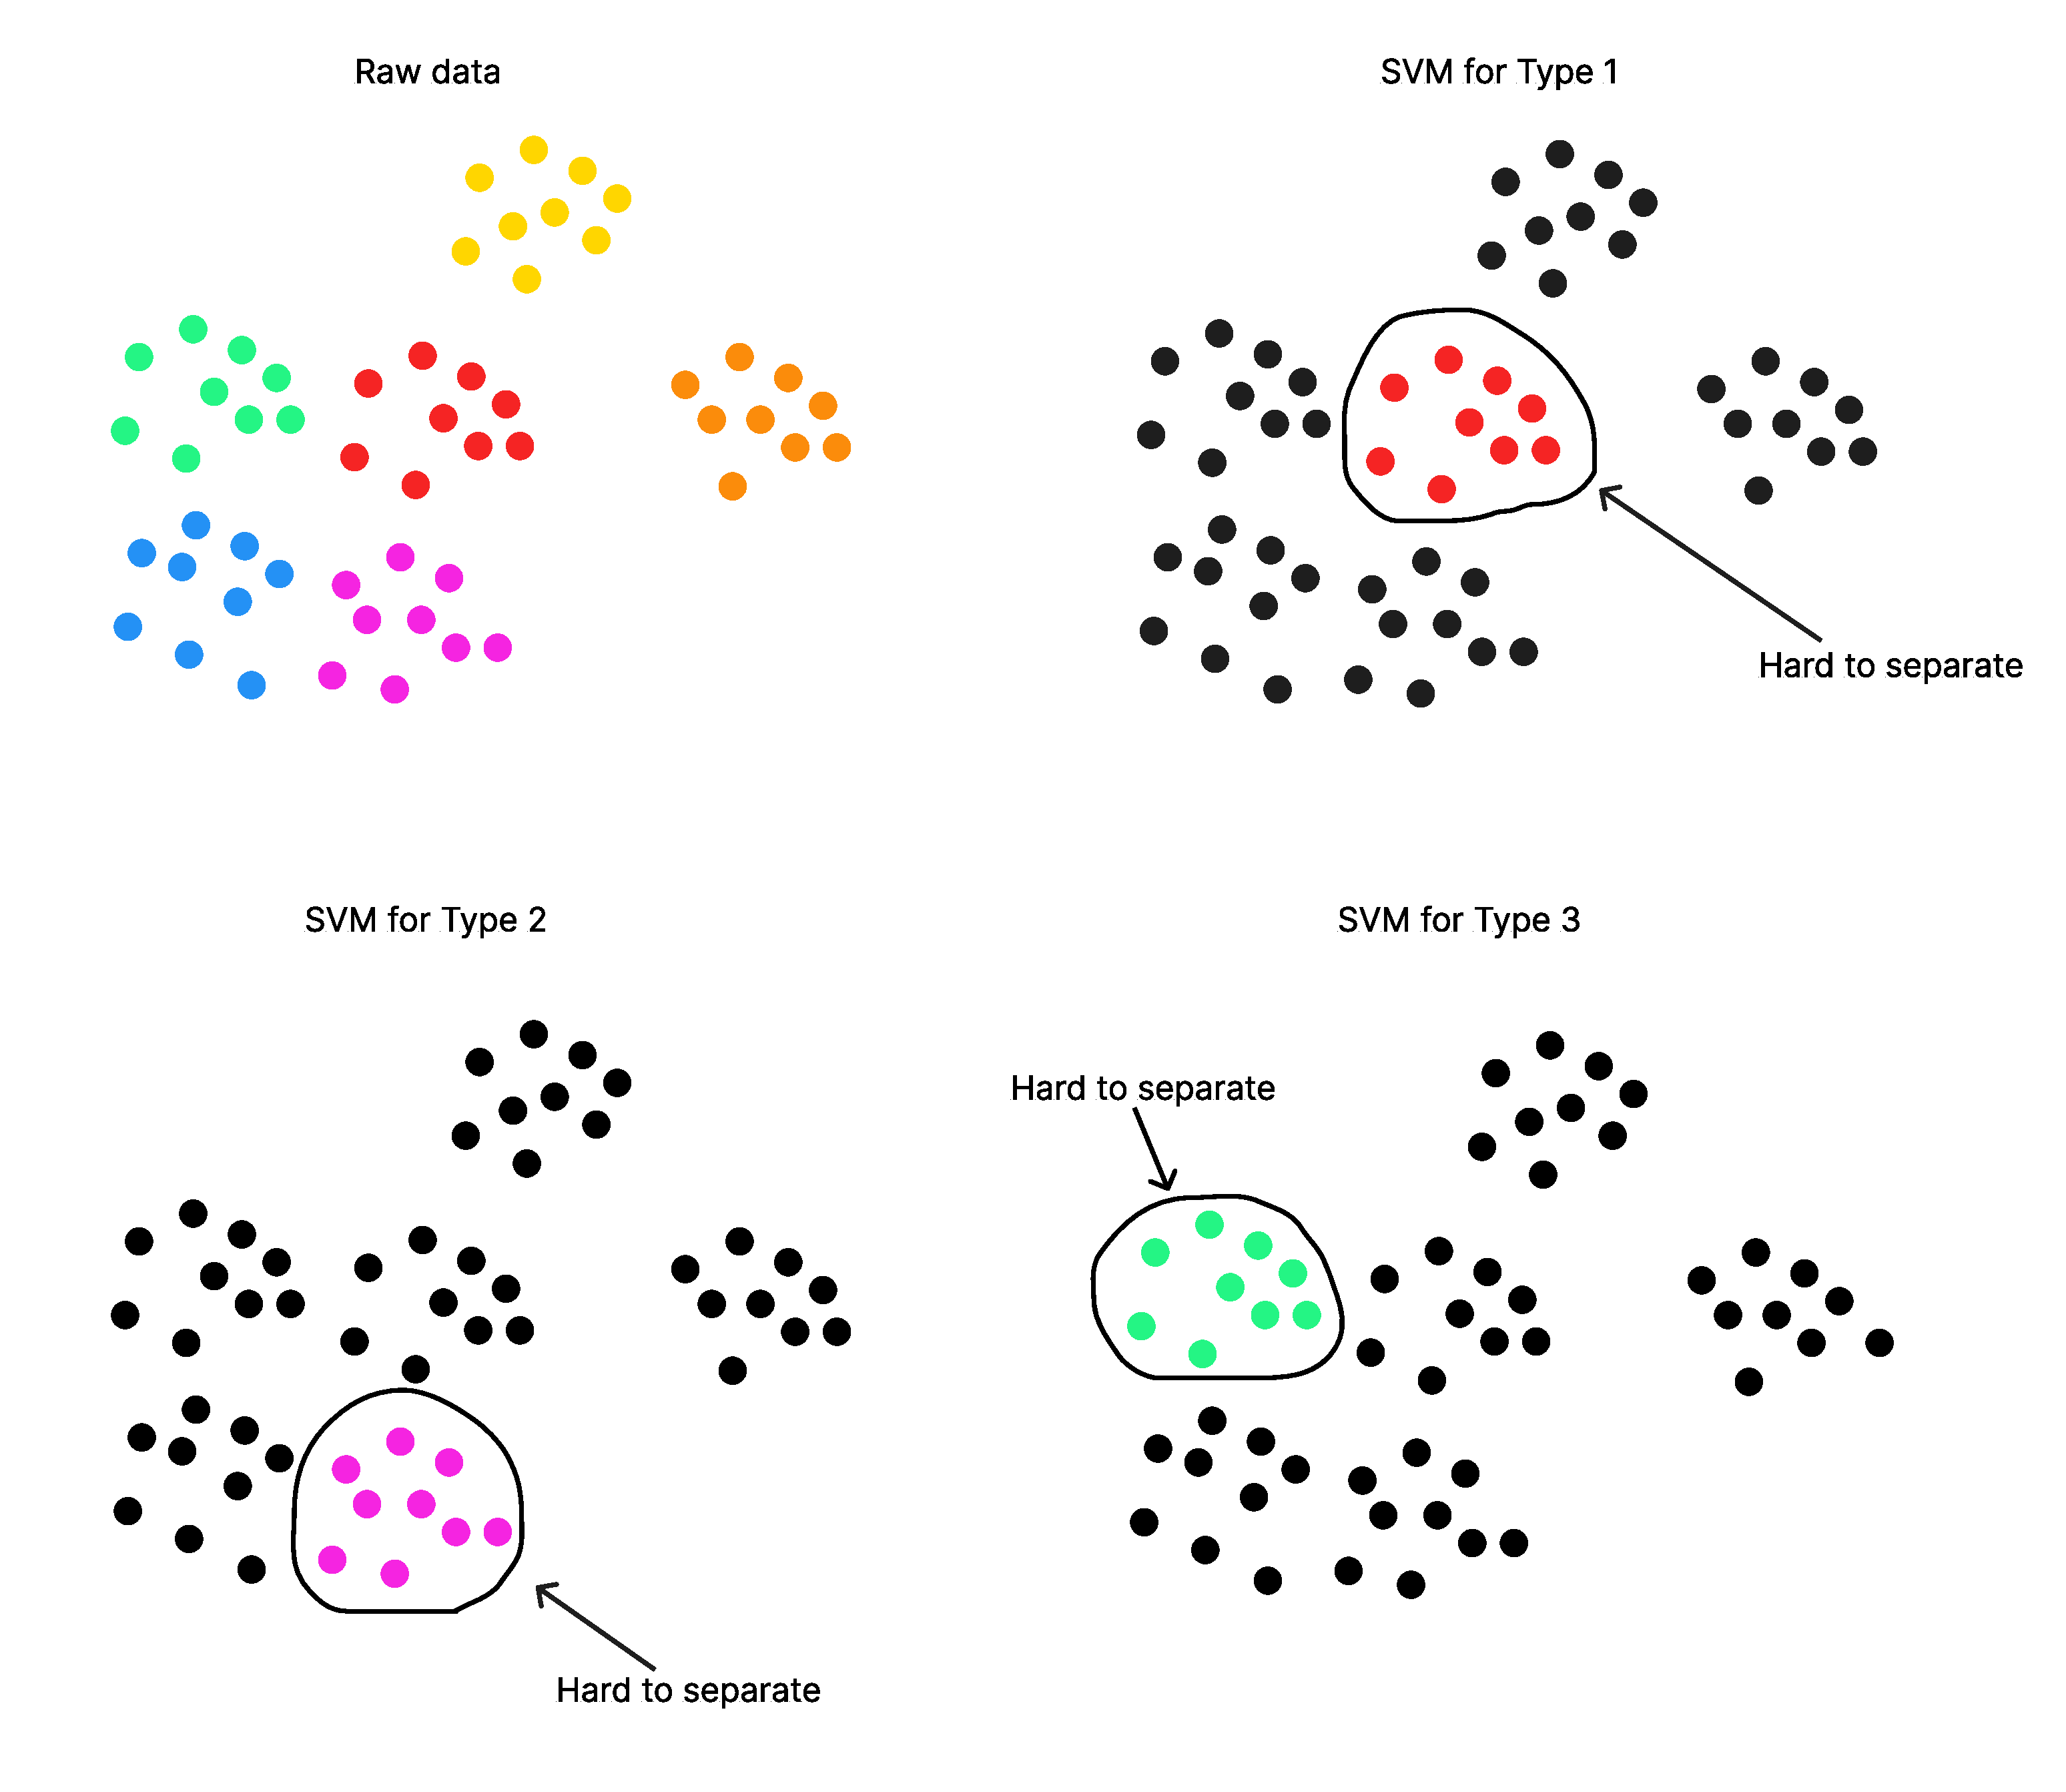
\includegraphics[scale=0.15]{assets/SVM_fail.pdf}
    \caption{An example that mult-classification SVMs fail}
    \label{fig:SVM_fail}
  \end{figure}

  In the other hand, KNN performs extraordinarily. In arrhythmia dataset, KNN with k-means in raw data gets 53.1646\% 
  accuracy, which is the highest accuracy comparing to others methods. And in gene expression cancer RNA-Seq dataset, 
  KNN with k-means in PCA data gets 94.8795\%. And KNN with DBSCAN performs well too. This method shows similar performance 
  in these two datasets, which also gets 94.5783\% in gene expression cancer RNA-Seq dataset PCA data. 

  For the NN part, SVDD cannot be trained with data only processed interpolation or PCA and AE with low dimension. The hypersphere that the SVDD defines will include or exclude almost all the data in the test dataset, which make the clustering almost impossible.
  On the other hand,SVDD can be trained with PCA-100-dimension data with accuracy up to 98 percent. With the NN with 100 percent accuracy and clustering algorithm NN-chain processing gene expression cancer RNA-Seq dataset,the accuray can achieve 75 percent correctness.

  \begin{table*}[tb]
    \newcommand{\z}{\phantom{0}}
    \caption{\textsc{Comparison of Classification Techniques. (Arrhythmia dataset)}}
      \vspace{-\baselineskip}
    \resizebox{\textwidth}{!}{
      \begin{tabular}{@{}lcccccccccccc@{}}\toprule
        Method                    & \multicolumn{2}{c}{Raw}                     & \multicolumn{2}{c}{Normalized}   & \multicolumn{2}{c}{PCA-32}        & \multicolumn{2}{c}{PCA-32 Normalized} & \multicolumn{2}{c}{AE-32}        & \multicolumn{2}{c}{AE-32 Normalized} \\ 
        \cmidrule(lr){2-3}\cmidrule(lr){4-5}\cmidrule(lr){6-7}\cmidrule(lr){8-9}\cmidrule(lr){10-11}\cmidrule(lr){12-13}
                                  & Search (s) & acc                            & Search (s) & acc                 & Search (s) & acc                  & Search (s) & acc                      & Search (s) & acc                  & Search (s) & acc            \\ \midrule
      KNN-Brute-Force + DBSCAN    & $0.0285$   & $47.4684 \pm 0$                & $0.0254$   & $46.8354 \pm 0$     & $0.0070$   & $38.6076 \pm 0$      & $0.0071$   & $42.4051\pm 0$           & $0.0071$   & $\bf{37.9747} \pm 0$ & $0.0071$   & $\bf{44.3038} \pm 0$\\
      SVM (linear) + DBSCAN       & $1.7269$   & $25.9494 \pm 0$                & $8.9285$   & $35.4430 \pm 0$     & $0.2186$   & $32.2785 \pm 0$      & $0.8162$   & $29.7468 \pm 0$          & $0.2169$   & $31.6456 \pm 0$      & $0.1552$   & $27.8481 \pm 0$\\
      SVM (polynomial) + DBSCAN   & $0.9993$   & $25.9494 \pm 0$                & $1.6100$   & $25.3165 \pm 0$     & $0.1997$   & $\z{1.2658} \pm 0$   & $0.4577$   & $33.5443 \pm 0$          & $0.2402$   & $30.3797 \pm 0$      & $0.4924$   & $30.2785 \pm 0$\\
      SVM (RBF) + DBSCAN          & $0.9915$   & $25.9494 \pm 0$                & $1.4681$   & $22.7848 \pm 0$     & $1.4328$   & $\z{0.6329} \pm 0$   & $11.9417$  & $30.3797 \pm 0$          & $13.5147$  & $22.1519 \pm 0$      & $24.7346$  & $34.1772 \pm 0$\\
      SVM (sigmoid) + DBSCAN      & $3.5272$   & $28.4810 \pm 0$                & $6.4731$   & $20.2532 \pm 0$     & $1.5779$   & $30.3797 \pm 0$      & $0.9797$   & $36.0759 \pm 0$          & $0.5284$   & $22.1519 \pm 0$      & $0.8430$   & $24.6835 \pm 0$\\
      KNN-Brute-Force + kmeans    & $0.0236$   & $\bf{53.1646} \pm 0$           & $0.0343$   & $\bf{50.6329} \pm 0$& $0.0068$   & $\bf{43.0380} \pm 0$ & $0.0069$   & $\bf{43.0380} \pm 0$     & $0.0069$   & $36.0759 \pm 0$      & $0.0080$   & $41.7722 \pm 0$\\
      SVM (linear) + kmeans       & $1.7719$   & $25.3165 \pm 0$                & $37.9747$  & $37.9747 \pm 0$     & $0.2317$   & $25.3165 \pm 0$      & $0.8932$   & $27.8481 \pm 0$          & $0.2331$   & $24.0506 \pm 0$      & $0.1596$   & $20.2532 \pm 0$\\
      SVM (polynomial) + kmeans   & $1.0456$   & $25.3165 \pm 0$                & $1.4942$   & $26.5823 \pm 0$     & $0.2326$   & $14.5570 \pm 0$      & $0.4094$   & $28.4810 \pm 0$          & $0.2033$   & $24.0506 \pm 0$      & $0.4884$   & $25.3165 \pm 0$\\
      SVM (RBF) + kmeans          & $34.5382$  & $\z{8.8608} \pm 0$             & $43.0936$  & $29.7468 \pm 0$     & $110.589$  & $\z{0.6329} \pm 0$   & $112.945$  & $\z{1.2658} \pm 0$       & $38.7497$  & $22.7848 \pm 0$      & $14.1561$  & $27.2152 \pm 0$\\
      SVM (sigmoid) + kmeans      & $4.0277$   & $22.6582 \pm 0$                & $8.0918$   & $17.7848 \pm 0$     & $0.7529$   & $25.3165 \pm 0$      & $0.7967$   & $12.0253 \pm 0$          & $0.6921$   & $17.7215 \pm 0$      & $0.4013$   & $28.4810 \pm 0$\\     
      NN + NNChain                & $0.6338$   & $31.6456 \pm 0$                & $0.633 $   & $29.7468 \pm 0$     & $0.9358$   & $31.6456 \pm 0$      & $0.8370$   & $30.3797 \pm 0$          & $1.0540$   & $29.7468 \pm 0$      & $1.0540$   & $29.7468 \pm 0$\\
      \bottomrule
      \end{tabular}
    }
    \label{table:Arrhythmia_result}
      \vspace{-\baselineskip}
  \end{table*}

  \begin{table*}[tb]
    \newcommand{\z}{\phantom{0}}
    \caption{\textsc{Comparison of Classification Techniques. (gene expression cancer RNA-Seq dataset)}}
      \vspace{-\baselineskip}
    \resizebox{\textwidth}{!}{
      \begin{tabular}{@{}lcccccccccccc@{}}\toprule
        Method                  & \multicolumn{2}{c}{Raw}        & \multicolumn{2}{c}{Normalized}     & \multicolumn{2}{c}{PCA-30}                & \multicolumn{2}{c}{PCA-30 Normalized} & \multicolumn{2}{c}{AE-30}         & \multicolumn{2}{c}{AE-30 Normalized} \\ 
        \cmidrule(lr){2-3}\cmidrule(lr){4-5}\cmidrule(lr){6-7}\cmidrule(lr){8-9}\cmidrule(lr){10-11}\cmidrule(lr){12-13}
                                & Search (s) & acc               & Search (s) & acc                   & Search (s) & acc                          & Search (s) & acc                      & Search (s) & acc                  & Search (s) & acc            \\ \midrule
      KNN-Brute-Force + DBSCAN  & $14.5101$  & $59.0361 \pm 0$   & $10.3013$  & $\bf{66.5663} \pm 0$  & $0.0224$   & $94.5783 \pm 0$              & $0.0237$   & $78.3133 \pm 0$          & $0.0258$   & $\bf{64.4578} \pm 0$ & $0.0235$   & $59.3373 \pm 0$\\
      SVM (linear) + DBSCAN     & $124.593$  & $61.7470 \pm 0$   & $610.6730$ & $\z{9.9398} \pm 0$    & $0.6466$   & $\z{9.9398} \pm 0$           & $0.1193$   & $10.5422 \pm 0$          & $0.1407$   & $63.2530 \pm 0$      & $0.1122$   & $13.5542 \pm 0$\\
      SVM (polynomial) + DBSCAN & $81.6495$  & $61.7470 \pm 0$   & $86.6406$  & $\z{1.2048} \pm 0$    & $0.2585$   & $64.4578 \pm 0$              & $0.3012$   & $61.1446 \pm 0$          & $0.2013$   & $63.2530 \pm 0$      & $0.2056$   & $50.3012 \pm 0$\\
      SVM (RBF) + DBSCAN        & $X$        & $\text{not converge}$ & $X$    & $\text{not converge}$ & $12.5077$  & $\z{9.9398} \pm 0$           & $3.8838$   & $63.2530 \pm 0$          & $5.0461$   & $40.3614 \pm 0$      & $11.4194$  & $49.6988 \pm 0$\\
      SVM (sigmoid) + DBSCAN    & $X$        & $\text{not converge}$ & $X$    & $\text{not converge}$ & $0.6372$   & $71.6867 \pm 0$              & $0.8222$   & $65.9639 \pm 0$          & $0.6236$   & $44.2771 \pm 0$      & $0.2273$   & $38.2530 \pm 0$\\
      KNN-Brute-Force + kmeans  & $22.754$   & $\bf{74.0964} \pm 0$& $6.36577$& $53.6145 \pm 0$       & $0.0212$   & $\bf{94.8795} \pm 0$         & $0.0214$   & $\bf{84.9398} \pm 0$     & $0.0214$   & $42.1687 \pm 0$      & $0.0220$   & $\bf{65.9639} \pm 0$\\
      SVM (linear) + kmeans     & $136.408$  & $61.7470 \pm 0$   & $664.2860$ & $\z{9.9398} \pm 0$    & $0.5914$   & $\z{9.9398} \pm 0$           & $0.1077$   & $10.5422 \pm 0$          & $0.1274$   & $63.2530 \pm 0$      & $0.1084$   & $13.2530 \pm 0$\\
      SVM (polynomial) + kmeans & $81.4276$  & $61.7470 \pm 0$   & $81.1669$  & $63.8554 \pm 0$       & $0.2003$   & $64.4578 \pm 0$              & $0.2167$   & $25.3012 \pm 0$          & $0.1780$   & $63.2530 \pm 0$      & $0.1930$   & $50.3012 \pm 0$\\
      SVM (RBF) + kmeans        & $1772.32$  & $\z{9.9398} \pm 0$& $1800.6$   & $\z{9.9398} \pm 0$    & $1.3625$   & $\z{9.9398} \pm 0$           & $1.3848$   & $\z{9.9398} \pm 0$       & $11.1729$  & $39.7590 \pm 0$      & $4.7882$   & $28.6145 \pm 0$\\
      SVM (sigmoid) + kmeans    & $190.866$  & $26.5060 \pm 0$   & $81.7487$  & $63.8554 \pm 0$       & $0.8287$   & $65.9639 \pm 0$              & $0.4269$   & $65.9639 \pm 0$          & $0.9908$   & $28.9157 \pm 0$      & $0.2360$   & $39.4578 \pm 0$\\
      NN + NNChain              & $163.359$  & $40.96   \pm 0$   & $169.031$  & $41.2651 \pm 0$       & $1.1779$   & $35.5421 \pm 0$              & $1.1170$   & $40.96 \pm 0$            & $0.9979$   & $16.4634 \pm 0$      & $1.0220$   & $41.2651 \pm 0$\\
      \bottomrule
      \end{tabular}
    }
    \label{table:gene_expression_result}
      \vspace{-\baselineskip}
  \end{table*}
  
\section{Conclusion}
In this study, we present a framework of algorithm to deal with the dataset containing 
out-of-knowledge data. And with in this algorithm, multiple major machine learning 
techniques are used, e.g., for preprocess, PCA, AE, normalization; for classification, 
KNN, SVM, SVDD, NN, as for clustering, DBSCAN, k-means, NN-chain. Among the various 
combinations, PCA + KNN + k-means performs outstanding in gene expression cancer RNA-Seq 
dataset, and raw data + KNN + k-means performs the best in arrhythmia dataset. Accidently, 
SVM performs bad in these two dataset. The main cause is the defect of the multi-classification 
SVMs design, which make some SVMs hard to separate the target types. However, by customize 
the kernel for each SVM, the problem may ease. In the same time, the increasing number of 
parameters can be fine-tuned by metaheuristic algorithms, e.g., simulated annealing, genetic 
algorithm, etc. We will develope a refinement design on multi-classification SVMs, to enhance 
the accuracy on these datasets.

\section{Contribution}
\begin{itemize}
  \item Hsieh Cheng-Han: KNN, SVM, DBSCAN, paper, ppt
  \item Hsu Ting-Hao: NN, SVDD, NN-Chain, paper, ppt
  \item Sun Shih-Yu: SVM, k-means, paper
  \item Lu Che-Yuan: 
  \item Huang Chia-Yen: Bayes, paper, poster
\end{itemize}

\bibliographystyle{IEEEtran}
\bibliography{main}
\end{document}

